\documentclass[9pt, twocolumn, a4paper]{jsarticle_kijou}
%
\usepackage{amsmath,amssymb}
\usepackage{bm}
\usepackage[dvipdfmx]{graphicx}
\usepackage{ascmac}
\usepackage[deluxe]{otf} 
\usepackage[margin=19mm]{geometry}

%%%% タイトルのフォント設定
\makeatletter
\renewcommand{\title}[1]{\gdef\@title{\bfseries\sffamily#1}}
\makeatother

\title{上半身ヒューマノイドロボットによる胴体を活用した投球}
\author{
4年8組11番 奥村 健人\\ % 名前
明治大学 理工学部 機械情報工学科 複雑ロボットシステム研究室\\ %所属
指導教員 新山 龍馬 % 指導教員
}
\date{}
\pagestyle{empty}
\begin{document}
\maketitle


\section{はじめに}
ロボットに投球を行わせる試みにおいて、人間の運動に見られるkinetic-chain(運動連鎖)をロボットアームに適用することで、腕のみながらも高速かつ高精度な結果を示した例1)や、ヒューマノイドロボットの全身を制御して行った投球で精度を向上させた例2)、人間の投球動作に基づいた姿勢からロボットの投球中のモーションを生成した例3)などがある。その一方で、これらを両立させ、人間と同等あるいはそれ以上の速度や精度での投球と、人間のように全身を協調させて動作させた投球を同時に行うことができた研究は見られない。\par
本研究では上半身型のヒューマノイドロボットを製作し、胴体を活用した協調動作による投球を行うことで、先行例で独立して達成されていた「高速・高精度な投球」と「人間らしい動作」を兼ね備えた結果を示すことを目的とする。これによって、ロボットの投球動作から人間への改善点のフィードバックや、人間対ロボットあるいは人間が操作するロボット同士で競うロボットスポーツなどの新形態の娯楽の発展が期待できる。\par

\section{使用したロボットと投球動作の実装}
\subsection{ロボットの仕様}
\begin{figure}[tbp]
  \centering
  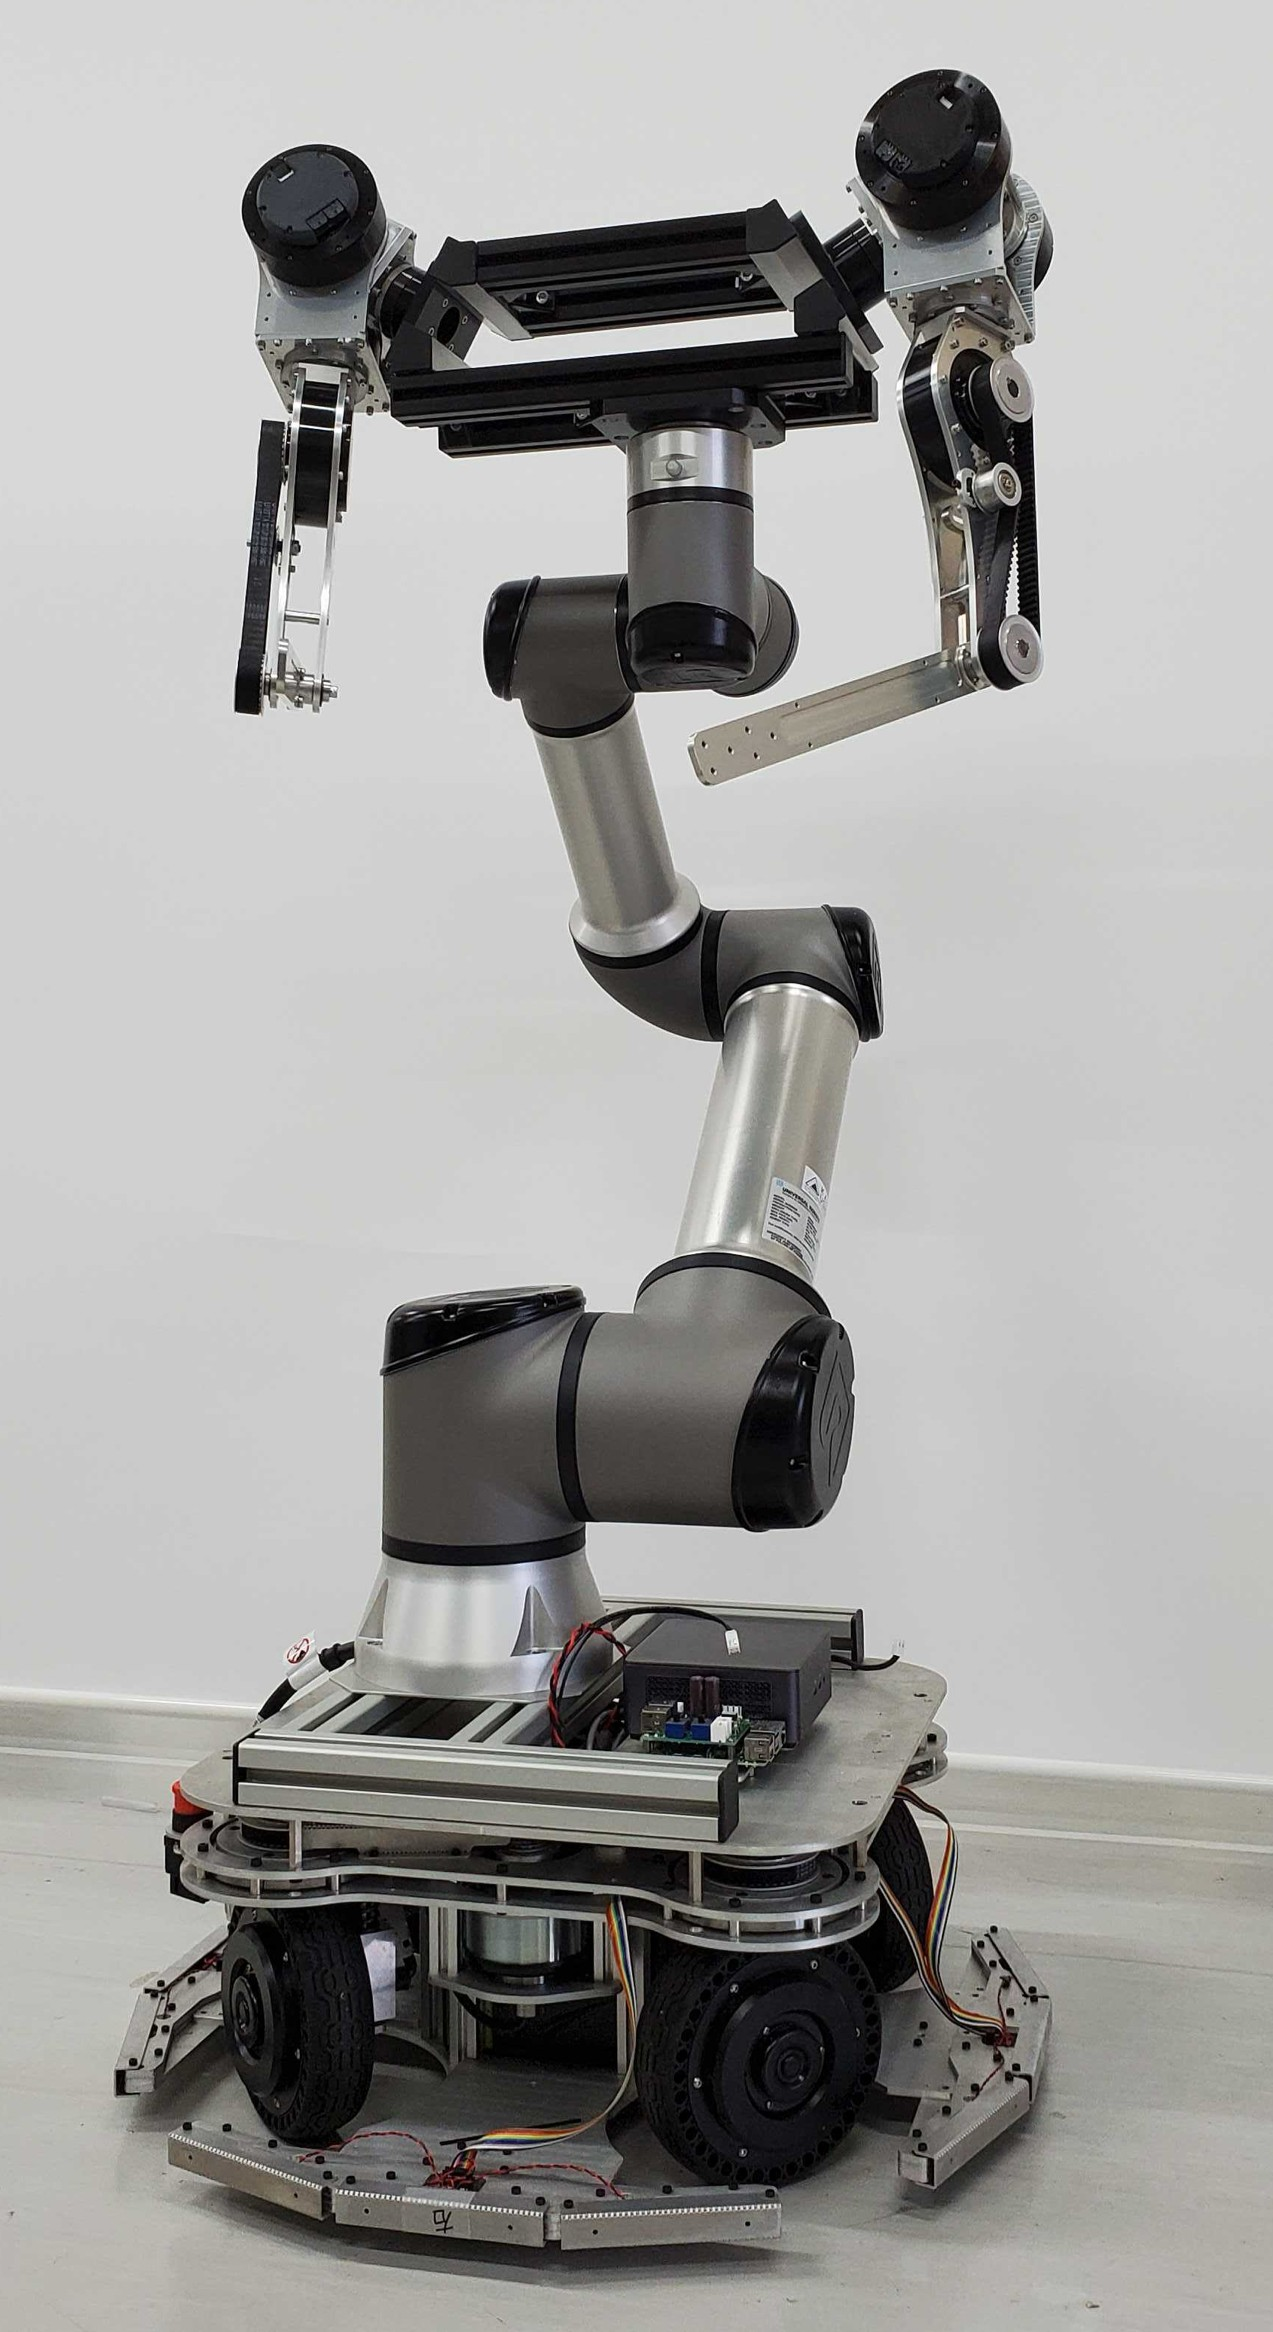
\includegraphics[height=0.4\textheight]{fig/img_wholebody.jpg}
  \caption{使用したロボット}
  \label{figure:img_wholebody}
 \end{figure}
 \begin{figure}[tbp]
  \centering
  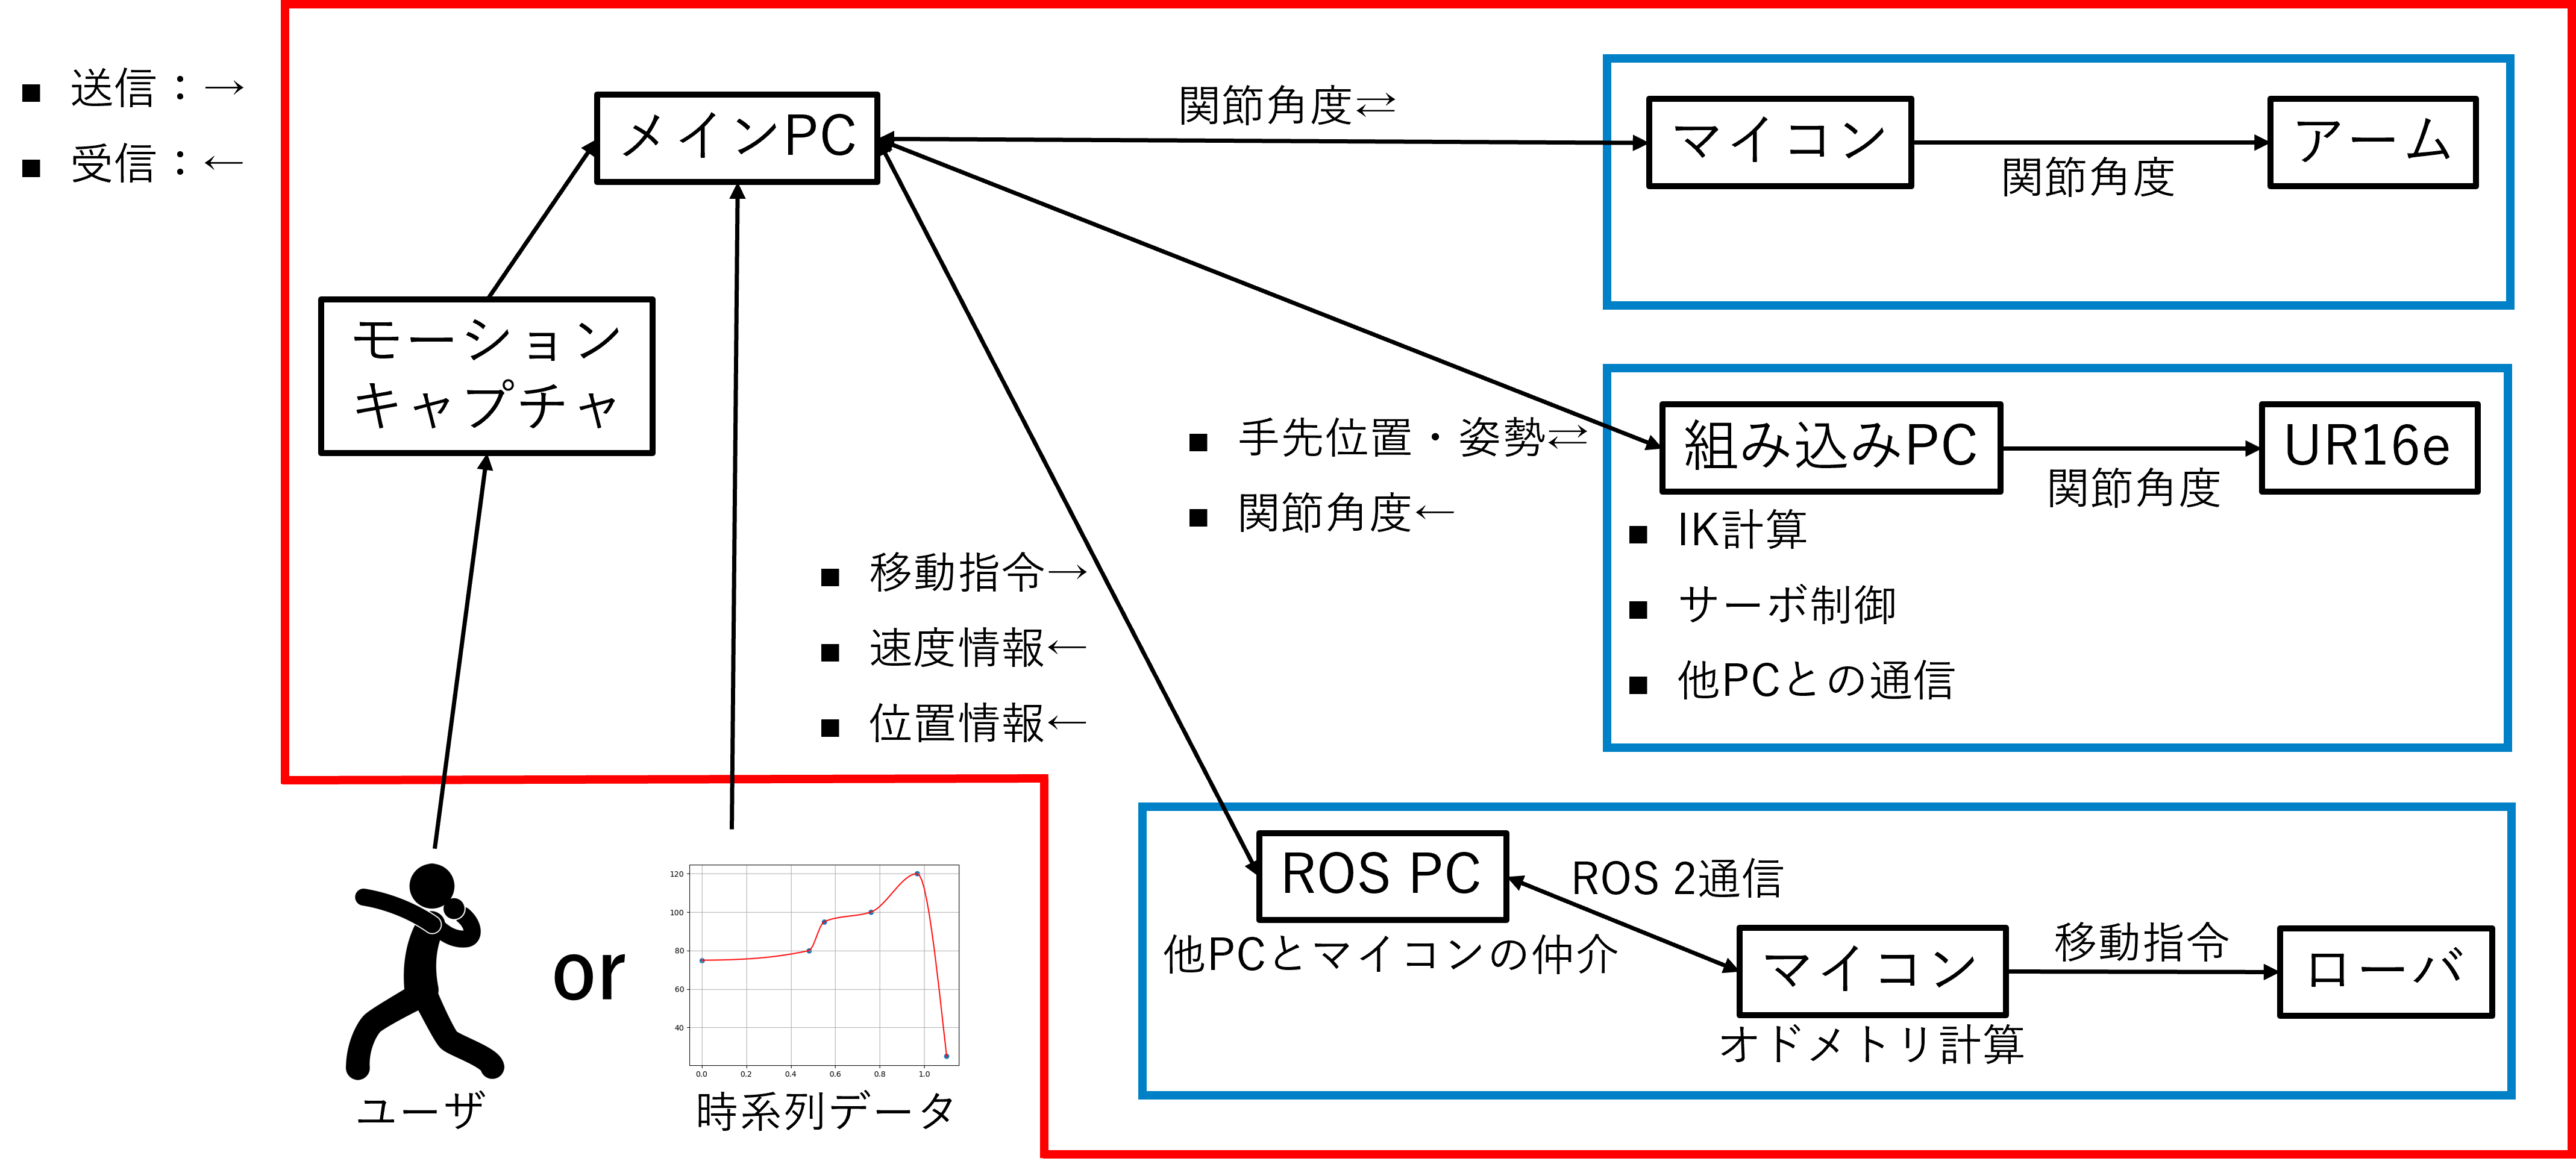
\includegraphics[width=0.48\textwidth]{fig/system_block.png}
  \caption{システム構成図}
  \label{figure:system_block}
 \end{figure}
本研究のために製作したロボットの全体像を\textbf{図1}に示す。ロボットは準ダイレクトドライブモータによる高速動作が可能な4DoFアーム、双腕を支えて6DoFでその位置・姿勢を決定できる協働ロボットアーム(UR16e, Universal Robots)、独立したステアリング軸を持ち全方向移動が可能な4輪ローバ(X120A, Vstone)で構成されている。\textbf{図2}に示すシステム構成図のように、これらのパーツと有線接続されたメインPCとがそれぞれで独立に通信を行い、並列で全身を制御する。\par

\subsection{投球モーションの生成}
本研究でロボットに行わせる投球モーションは、事前に用意した時系列データの入力によって生成する。入力データは人間の投球動作について調査された文献4)、5)のうち、投球中の複数タイミングでの主要な関節の角度の数値をもとに、元の動作の軌道の滑らかさを保持するために区分3次エルミート補間によって作成した。今回は、胴体のUR16eの姿勢のうち$y$軸まわりと$z$軸まわりの変化と、腕の4つのモータの角度変化の、合計6種類の時系列データを用意した。ただし、ロボットの正面を$x$軸、鉛直上向きを$z$軸とする右手系とする。\par

\section{ロボットによる投球実験}
\subsection{腕のみの場合と協調動作を行った場合の比較}
本実験では準備した時系列データを用いて、腕のみを動かした場合と胴体との協調動作を行った場合で投球を行った。ただし胴体が動いてから腕が動くまでの遅延の秒数をパラメータとして0.1~sずつ変化させ、4.0-4.6~sの7段階で3回ずつ実験した。これらの合計8パターンの条件での投球実験において、腕の先端に取り付けたマーカの位置を計測し、計測フレーム間の位置差から手先の速さを計算し、比較を行った。この実験によって腕と胴体の協調動作の効果を測ることを目的とした。\par

\subsection{実験結果}
\begin{table}[tbp]
  \centering
  \caption{条件ごとの最大手先速さ}
  \label{tab:result_max_val}
  \begin{tabular}{cc}
    \hline
    Condition & Max speed average$\,$($\pm$SD)\\
     & (m/s)\\
    \hline
    Only arm & $3.53\,(\pm0.06)$\\
    4.0~s & $4.44\,(\pm0.12)$\\
    4.1~s & $4.37\,(\pm0.20)$\\
    4.2~s & $4.45\,(\pm0.10)$\\
    4.3~s & $4.49\,(\pm0.17)$\\
    4.4~s & $4.41\,(\pm0.15)$\\
    4.5~s & $4.30\,(\pm0.10)$\\
    4.6~s & $4.51\,(\pm0.04)$\\
    \hline
  \end{tabular}
\end{table}
紙面の都合上実験で得られたグラフを全て載せることができないため、代わりに\textbf{表1}に条件ごとの最大手先速さの平均値と標準偏差をまとめた。\par

\subsection{結果についての考察}
表1から、腕のみの場合に比べて胴体を含んだ動作による投球のいずれも手先の速さが向上することが分かる。一方、腕が動き始めるタイミングによって顕著に数値が向上した条件は見られず、突出して適した条件は確認できなった。これは、胴体として動かしたUR16eの動作速度が想定よりも遅かったことが主な原因と考えられる。すなわち、胴体の動きが制限下での最高速度であったために、腕の動作に対して一定速度が加えられるだけになってしまったと推察される。\par
標準偏差について、概ね$\pm0.10$~m/s前後だが4.1~sや4.3~sの場合に若干ばらつきが大きくなっている。これは腕が伸びてモーメントアームが大きくなったタイミングの前後で、腕の動きによって発生する大きな振動をUR16eが検知してしまい動作を停止してしまったことが原因であり、この停止のタイミングが一定ではないために手先の最大速さにもばらつきが発生したと思われる。\par
本実験で確認された最大手先速さは$4.51\,(\pm0.04)$~m/sであったが、人間の投球時に発生する最大速さは文献では約31.6~m/sであった。また確認した先行研究の中で最も動作速度が大きかった例1)での最大速さは6~m/sであった。このことから、胴体を含む投球の結果は腕のみの先行研究などのロボットの投球や、本物の人間にはまだ及んでいないと言える。この原因の一つとして、モーションが人間を参考としている一方で、筋肉や腱による人間の身体の弾性などの動力学特性を再現することができなかったことが挙げられる。\par

\section{まとめ}
本研究は、ロボットの投球における高速・高精度な結果と人間のような動作を、人間の投球動作を参考にした胴体を活用した投球モーションの生成によって実現することを目標として行われた。これによってアバターロボットによる人間と同等かそれ以上の投球を実現すれば、指導用のツールとしての使用やロボットスポーツなどの新形態の娯楽への寄与が期待できる。具体的な手法として、上半身型ヒューマノイドロボットの開発と投球実験を行った。ロボットは投球という目的に合うと考えた要素を組み合わせ、人間の投球動作に関する複数の文献から作成したデータをロボットに入力することで投球モーションを生成した。\par
実験の結果、腕のみで行う投球に比べて胴体と協調した動作によってより大きな手先の速さを発生させることができることが確認できた。しかし、腕の動作タイミングによる結果の違いに顕著な違いは確認できなった。また、今回の結果は実際の人間が発生させる値には及ばず、これは動力学的な要素の再現ができていないことが大きな原因であると考えられる。これに加えて、胴体に用いたマニピュレータの動作速度不足や、保護停止機能による結果のばらつきは致命的な問題であり、目下解決するべき課題であると言える。\par


\section*{\small 参考文献}{
\small
\begin{enumerate}
\renewcommand{\labelenumi}{\arabic{enumi}).}
  \item T. Senoo, A. Namiki and M. Ishikawa, "High-speed throwing motion based on kinetic chain approach," in 2008 IEEE/RSJ International Conference on Intelligent Robots and Systems. IEEE, 2008, pp.3206–3211.
  \item T. H. S. Li, P. H. Kuo, C. Y. Chang, H. P. Hsu, Y. C. Chen, and C. H. Chang, "Deep belief network–based learning algorithm for humanoid robot in a pitching game," IEEE Access, vol.7, pp.165659–165670, 2019.
  \item D. M. Lofaro, C. Sun and P. Oh, "Humanoid pitching at a major league baseball game: Challenges, approach, implementation and lessons learned," in 2012 12th IEEE-RAS International Conference on Humanoid Robots (Humanoids 2012). IEEE, 2012, pp.423–428.
  \item G. J. Calabrese, "Pitching mechanics, revisited," International journal of sports physical therapy, vol.8, no.5, p.652, 2013.
  \item M. Kageyama, T. Sugiyama, Y. Takai, H. Kanehisa and A. Maeda, "Kinematic and kinetic profiles of trunk and lower limbs during baseball pitching in collegiate pitchers," Journal of
  sports science \& medicine, vol.13, no.4, p.742, 2014.
\end{enumerate}
}

\end{document}